\chapter{Magic}
\section{Casting Spells}

\label{f0}				
Whether a spell is arcane or divine, and whether a character prepares spells in advance or chooses them on the spot, casting a spell works the same way.
				
\subsection{Choosing a Spell}

				
First you must choose which spell to cast. If you're a cleric, druid, experienced paladin, experienced ranger, or wizard, you select from among spells prepared earlier in the day and not yet cast (see Preparing Wizard Spells and Preparing Divine Spells).
				
If you're a bard or sorcerer, you can select any spell you know, provided you are capable of casting spells of that level or higher.
				
To cast a spell, you must be able to speak (if the spell has a verbal component), gesture (if it has a somatic component), and manipulate the material components or focus (if any). Additionally, you must concentrate to cast a spell. 
				
If a spell has multiple versions, you choose which version to use when you cast it. You don't have to prepare (or learn, in the case of a bard or sorcerer) a specific version of the spell.
				
Once you've cast a prepared spell, you can't cast it again until you prepare it again. (If you've prepared multiple copies of a single spell, you can cast each copy once.) If you're a bard or sorcerer, casting a spell counts against your daily limit for spells of that spell level, but you can cast the same spell again if you haven't reached your limit.
				
\subsection{Concentration}

\begin{table}
 \sffamily
 \caption{Concentration Check DCs}
 \begin{tabular}{ll}
\textbf{Situation} & \textbf{Concentration Check DC}\\
Cast defensively & 15 + double spell level\\
Injured while casting & 10 + damage dealt\\
                      & + spell level\\
Continuous damage while casting & 10 + 1/2 damage dealt \\
                                & + spell level\\
Affected by a non-damaging spell & DC of the spell\\
 while casting                    & + spell level\\
Grappled or pinned while casting & 10 + grappler's CMB \\
                                 & + spell level\\
Vigorous motion while casting & 10 + spell level\\
Violent motion while casting & 15 + spell level\\
Extremely violent motion while & 20 + spell level\\
casting & \\
Wind with rain or sleet while& 5 + spell level\\
 casting & \\
Wind with hail and debris while& 10 + spell level\\
 casting & \\
Weather caused by spell & see spell\\
Entangled while casting & 15 + spell level\\
 \end{tabular}

\end{table}


				
To cast a spell, you must concentrate. If something interrupts your concentration while you're casting, you must make a concentration check or lose the spell. When you make a concentration check, you roll d20 and add your caster level and the ability score modifier used to determine bonus spells of the same type. Clerics, druids, and rangers add their Wisdom modifier. Bards, paladins, and sorcerers add their Charisma modifier. Finally, wizards add their Intelligence modifier. The more distracting the interruption and the higher the level of the spell you are trying to cast, the higher the DC (see Table: Concentration Check DCs). If you fail the check, you lose the spell just as if you had cast it to no effect.
				
\textbf{Injury}: If you take damage while trying to cast a spell, you must make a concentration check with a DC equal to 10 + the damage taken + the level of the spell you're casting. If you fail the check, you lose the spell without effect. The interrupting event strikes during spellcasting if it comes between the time you started and the time you complete a spell (for a spell with a casting time of 1 full round or more) or if it comes in response to your casting the spell (such as an attack of opportunity provoked by the spell or a contingent attack, such as a readied action).
				
If you are taking continuous damage, such as from an \textit{acid arrow} or by standing in a lake of lava, half the damage is considered to take place while you are casting a spell. You must make a concentration check with a DC equal to 10 + 1/2 the damage that the continuous source last dealt + the level of the spell you're casting. If the last damage dealt was the last damage that the effect could deal, then the damage is over and does not distract you.
				
\textbf{Spell}: If you are affected by a spell while attempting to cast a spell of your own, you must make a concentration check or lose the spell you are casting. If the spell affecting you deals damage, the DC is 10 + the damage taken + the level of the spell you're casting.
				
If the spell interferes with you or distracts you in some other way, the DC is the spell's saving throw DC + the level of the spell you're casting. For a spell with no saving throw, it's the DC that the spell's saving throw would have if a save were allowed (10 + spell level + caster's ability score).
				
\textbf{Grappling or Pinned}: Casting a spell while you have the grappled or pinned condition is difficult and it requires a concentration check (DC 10 + the grappler's CMB + the level of the spell you're casting). Pinned creatures can only cast spells that do not have somatic components.
				
\textbf{Vigorous Motion}: If you are riding on a moving mount, taking a bouncy ride in a wagon, on a small boat in rough water, belowdecks in a storm-tossed ship, or simply being jostled in a similar fashion, you must make a concentration check (DC 10 + the level of the spell you're casting) or lose the spell. 
				
\textbf{Violent Motion}: If you are on a galloping horse, taking a very rough ride in a wagon, on a small boat in rapids or in a storm, on deck in a storm-tossed ship, or being pitched roughly about in a similar fashion, you must make a concentration check (DC 15 + the level of the spell you're casting) or lose the spell. If the motion is extremely violent, such as that caused by an earthquake, the DC is equal to 20 + the level of the spell you're casting.
				
\textbf{Violent Weather}: You must make a concentration check if you try to cast a spell in violent weather. If you are in a high wind carrying blinding rain or sleet, the DC is 5 + the level of the spell you're casting. If you are in wind-driven hail, dust, or debris, the DC is 10 + the level of the spell you're casting. In either case, you lose the spell if you fail the concentration check. If the weather is caused by a spell, use the rules as described in the spell's description.
				
\textbf{Casting Defensively}: If you want to cast a spell without provoking any attacks of opportunity, you must make a concentration check (DC 15 + double the level of the spell you're casting) to succeed. You lose the spell if you fail.
				
\textbf{Entangled}: If you want to cast a spell while entangled in a net or by a tanglefoot bag or while you're affected by a spell with similar effects, you must make a concentration check to cast the spell (DC 15 + the level of the spell you're casting). You lose the spell if you fail.
				
\subsection{Counterspells}

				
It is possible to cast any spell as a counterspell. By doing so, you are using the spell's energy to disrupt the casting of the same spell by another character. Counterspelling works even if one spell is divine and the other arcane.
				
\textbf{How Counterspells Work}: To use a counterspell, you must select an opponent as the target of the counterspell. You do this by choosing to ready an action. In doing so, you elect to wait to complete your action until your opponent tries to cast a spell. You may still move at your normal speed, since ready is a standard action.
				
If the target of your counterspell tries to cast a spell, make a Spellcraft check (DC 15 + the spell's level). This check is a free action. If the check succeeds, you correctly identify the opponent's spell and can attempt to counter it. If the check fails, you can't do either of these things.
				
To complete the action, you must then cast an appropriate spell. As a general rule, a spell can only counter itself. If you are able to cast the same spell and you have it prepared (or have a slot of the appropriate level available), you cast it, creating a counterspell effect. If the target is within range, both spells automatically negate each other with no other results.
				
\textbf{Counterspelling Metamagic Spells}: Metamagic feats are not taken into account when determining whether a spell can be countered.
				
\textbf{Specific Exceptions}: Some spells can counter other specific spells, often those with diametrically opposed effects.
				
\textbf{\textit{Dispel Magic } as a Counterspell}: You can usually use \textit{dispel magic }to counterspell another spell being cast without needing to identify the spell being cast. \textit{Dispel magic }doesn't always work as a counterspell (see the spell description).
				
\subsection{Caster Level}

				
A spell's power often depends on its caster level, which for most spellcasting characters is equal to her class level in the class she's using to cast the spell. 
				
You can cast a spell at a lower caster level than normal, but the caster level you choose must be high enough for you to cast the spell in question, and all level-dependent features must be based on the same caster level. 
				
In the event that a class feature or other special ability provides an adjustment to your caster level, that adjustment applies not only to effects based on caster level (such as range, duration, and damage dealt), but also to your caster level check to overcome your target's spell resistance and to the caster level used in dispel checks (both the dispel check and the DC of the check). 
				
\subsection{Spell Failure}

				
If you ever try to cast a spell in conditions where the characteristics of the spell cannot be made to conform, the casting fails and the spell is wasted.
				
Spells also fail if your concentration is broken and might fail if you're wearing armor while casting a spell with somatic components.
				
\subsection{The Spell's Result}

				
Once you know which creatures (or objects or areas) are affected, and whether those creatures have made successful saving throws (if any were allowed), you can apply whatever results a spell entails.
				
\subsection{Special Spell Effects}

				
Many special spell effects are handled according to the school of the spells in question. Certain other special spell features are found across spell schools.
				
\textbf{Attacks}: Some spell descriptions refer to attacking. All offensive combat actions, even those that don't damage opponents, are considered attacks. Attempts to channel energy count as attacks if it would harm any creatures in the area. All spells that opponents resist with saving throws, that deal damage, or that otherwise harm or hamper subjects are attacks. Spells that summon monsters or other allies are not attacks because the spells themselves don't harm anyone.
				
\textbf{Bonus Types}: Usually, a bonus has a type that indicates how the spell grants the bonus. The important aspect of bonus types is that two bonuses of the same type don't generally stack. With the exception of dodge bonuses, most circumstance bonuses, and racial bonuses, only the better bonus of a given type works (see Combining Magical Effects). The same principle applies to penalties---a character taking two or more penalties of the same type applies only the worst one, although most penalties have no type and thus always stack. Bonuses without a type always stack, unless they are from the same source.
				
\textbf{Bringing Back the Dead}: Several spells have the power to restore slain characters to life.
				
When a living creature dies, its soul departs its body, leaves the Material Plane, travels through the Astral Plane, and goes to abide on the plane where the creature's deity resides. If the creature did not worship a deity, its soul departs to the plane corresponding to its alignment. Bringing someone back from the dead involves magically retrieving his soul and returning it to his body. For more information on the planes, see Environment.
				
\textit{Negative Levels}: Any creature brought back to life usually gains one or more permanent negative levels (see Special Abilities). These levels apply a penalty to most rolls until removed through spells such as \textit{restoration}. If the character was 1st level at the time of death, he loses 2 points of Constitution instead of gaining a negative level.
				
\textit{Preventing Revivification}: Enemies can take steps to make it more difficult for a character to be returned from the dead. Keeping the body prevents others from using \textit{raise dead }or \textit{resurrection }to restore the slain character to life. Casting \textit{trap the soul }prevents any sort of revivification unless the soul is first released.
				
\textit{Revivification against One's Will}: A soul can't be returned to life if it doesn't wish to be. A soul knows the name, alignment, and patron deity (if any) of the character attempting to revive it and may refuse to return on that basis.
				
\subsection{Combining Magic Effects}

				
Spells or magical effects usually work as described, no matter how many other spells or magical effects happen to be operating in the same area or on the same recipient. Except in special cases, a spell does not affect the way another spell operates. Whenever a spell has a specific effect on other spells, the spell description explains that effect. Several other general rules apply when spells or magical effects operate in the same place:
				
\textbf{Stacking Effects}: Spells that provide bonuses or penalties on attack rolls, damage rolls, saving throws, and other attributes usually do not stack with themselves. More generally, two bonuses of the same type don't stack even if they come from different spells (or from effects other than spells; see Bonus Types, above). 
				
\textit{Different Bonus Types}: The bonuses or penalties from two different spells stack if the modifiers are of different types. A bonus that doesn't have a type stacks with any bonus.
				
\textit{Same Effect More than Once in Different Strengths}: In cases when two or more identical spells are operating in the same area or on the same target, but at different strengths, only the one with the highest strength applies.
				
\textit{Same Effect with Differing Results}: The same spell can sometimes produce varying effects if applied to the same recipient more than once. Usually the last spell in the series trumps the others. None of the previous spells are actually removed or dispelled, but their effects become irrelevant while the final spell in the series lasts.
				
\textit{One Effect Makes Another Irrelevant}: Sometimes, one spell can render a later spell irrelevant. Both spells are still active, but one has rendered the other useless in some fashion.
				
\textit{Multiple Mental Control Effects}: Sometimes magical effects that establish mental control render each other irrelevant, such as spells that remove the subject's ability to act. Mental controls that don't remove the recipient's ability to act usually do not interfere with each other. If a creature is under the mental control of two or more creatures, it tends to obey each to the best of its ability, and to the extent of the control each effect allows. If the controlled creature receives conflicting orders simultaneously, the competing controllers must make opposed Charisma checks to determine which one the creature obeys.
				
\textbf{Spells with Opposite Effects}: Spells with opposite effects apply normally, with all bonuses, penalties, or changes accruing in the order that they apply. Some spells negate or counter each other. This is a special effect that is noted in a spell's description. 
				
\textbf{Instantaneous Effects}: Two or more spells with instantaneous durations work cumulatively when they affect the same target.
				
\section{Spell Descriptions}

				
The description of each spell is presented in a standard format. Each category of information is explained and defined below.
				
\subsection{Name}

				
The first line of every spell description gives the name by which the spell is generally known.
				
\subsection{School (Subschool)}

				
Beneath the spell name is a line giving the school of magic (and the subschool, if any) to which the spell belongs.
				
Almost every spell belongs to one of eight schools of magic. A school of magic is a group of related spells that work in similar ways. A small number of spells (\textit{arcane mark, limited wish, permanency, prestidigitation, }and \textit{wish}) are universal, belonging to no school.
				
\subsection{Abjuration}

				
Abjurations are protective spells. They create physical or magical barriers, negate magical or physical abilities, harm trespassers, or even banish the subject of the spell to another plane of existence. 
				
If one abjuration spell is active within 10 feet of another for 24 hours or more, the magical fields interfere with each other and create barely visible energy fluctuations. The DC to find such spells with the Perception skill drops by 4.
				
If an abjuration creates a barrier that keeps certain types of creatures at bay, that barrier cannot be used to push away those creatures. If you force the barrier against such a creature, you feel a discernible pressure against the barrier. If you continue to apply pressure, you end the spell.
				
\subsection{Conjuration}

				
Each conjuration spell belongs to one of five subschools. Conjurations transport creatures from another plane of existence to your plane (calling); create objects or effects on the spot (creation); heal (healing); bring manifestations of objects, creatures, or forms of energy to you (summoning); or transport creatures or objects over great distances (teleportation). Creatures you conjure usually---but not always---obey your commands.
				
A creature or object brought into being or transported to your location by a conjuration spell cannot appear inside another creature or object, nor can it appear floating in an empty space. It must arrive in an open location on a surface capable of supporting it.
				
The creature or object must appear within the spell's range, but it does not have to remain within the range.
				
\textbf{Calling}: A calling spell transports a creature from another plane to the plane you are on. The spell grants the creature the one-time ability to return to its plane of origin, although the spell may limit the circumstances under which this is possible. Creatures who are called actually die when they are killed; they do not disappear and reform, as do those brought by a summoning spell (see below). The duration of a calling spell is instantaneous, which means that the called creature can't be dispelled.
				
\textbf{Creation}: A creation spell manipulates matter to create an object or creature in the place the spellcaster designates. If the spell has a duration other than instantaneous, magic holds the creation together, and when the spell ends, the conjured creature or object vanishes without a trace. If the spell has an instantaneous duration, the created object or creature is merely assembled through magic. It lasts indefinitely and does not depend on magic for its existence.
				
\textbf{Healing}: Certain divine conjurations heal creatures or even bring them back to life.
				
\textbf{Summoning}: A summoning spell instantly brings a creature or object to a place you designate. When the spell ends or is dispelled, a summoned creature is instantly sent back to where it came from, but a summoned object is not sent back unless the spell description specifically indicates this. A summoned creature also goes away if it is killed or if its hit points drop to 0 or lower, but it is not really dead. It takes 24 hours for the creature to reform, during which time it can't be summoned again.
				
When the spell that summoned a creature ends and the creature disappears, all the spells it has cast expire. A summoned creature cannot use any innate summoning abilities it may have.
				
\textbf{Teleportation}: A teleportation spell transports one or more creatures or objects a great distance. The most powerful of these spells can cross planar boundaries. Unlike summoning spells, the transportation is (unless otherwise noted) one-way and not dispellable.
				
Teleportation is instantaneous travel through the Astral Plane. Anything that blocks astral travel also blocks teleportation.
				
\subsection{Divination}

				
Divination spells enable you to learn secrets long forgotten, predict the future, find hidden things, and foil deceptive spells.
				
Many divination spells have cone-shaped areas. These move with you and extend in the direction you choose. The cone defines the area that you can sweep each round. If you study the same area for multiple rounds, you can often gain additional information, as noted in the descriptive text for the spell.
				
\textbf{Scrying}: A scrying spell creates an invisible magical sensor that sends you information. Unless noted otherwise, the sensor has the same powers of sensory acuity that you possess. This level of acuity includes any spells or effects that target you, but not spells or effects that emanate from you. The sensor, however, is treated as a separate, independent sensory organ of yours, and thus functions normally even if you have been blinded or deafened, or otherwise suffered sensory impairment.
				
A creature can notice the sensor by making a Perception check with a DC 20 + the spell level. The sensor can be dispelled as if it were an active spell.
				
Lead sheeting or magical protection blocks a scrying spell, and you sense that the spell is blocked.
				
\subsection{Enchantment}

				
Enchantment spells affect the minds of others, influencing or controlling their behavior.
				
All enchantments are mind-affecting spells. Two subschools of enchantment spells grant you influence over a subject creature.
				
\textbf{Charm}: A charm spell changes how the subject views you, typically making it see you as a good friend.
				
\textbf{Compulsion}: A compulsion spell forces the subject to act in some manner or changes the way its mind works. Some compulsion spells determine the subject's actions or the effects on the subject, others allow you to determine the subject's actions when you cast the spell, and still others give you ongoing control over the subject.
				
\subsection{Evocation}

				
Evocation spells manipulate magical energy or tap an unseen source of power to produce a desired end. In effect, an evocation draws upon magic to create something out of nothing. Many of these spells produce spectacular effects, and evocation spells can deal large amounts of damage.
				
\subsection{Illusion}

				
Illusion spells deceive the senses or minds of others. They cause people to see things that are not there, not see things that are there, hear phantom noises, or remember things that never happened.
				
\textbf{Figment}: A figment spell creates a false sensation. Those who perceive the figment perceive the same thing, not their own slightly different versions of the figment. It is not a personalized mental impression. Figments cannot make something seem to be something else. A figment that includes audible effects cannot duplicate intelligible speech unless the spell description specifically says it can. If intelligible speech is possible, it must be in a language you can speak. If you try to duplicate a language you cannot speak, the figment produces gibberish. Likewise, you cannot make a visual copy of something unless you know what it looks like (or copy another sense exactly unless you have experienced it).
				
Because figments and glamers are unreal, they cannot produce real effects the way that other types of illusions can. Figments and glamers cannot cause damage to objects or creatures, support weight, provide nutrition, or provide protection from the elements. Consequently, these spells are useful for confounding foes, but useless for attacking them directly. 
				
A figment's AC is equal to 10 + its size modifier.
				
\textbf{Glamer}: A glamer spell changes a subject's sensory qualities, making it look, feel, taste, smell, or sound like something else, or even seem to disappear.
				
\textbf{Pattern}: Like a figment, a pattern spell creates an image that others can see, but a pattern also affects the minds of those who see it or are caught in it. All patterns are mind-affecting spells.
				
\textbf{Phantasm}: A phantasm spell creates a mental image that usually only the caster and the subject (or subjects) of the spell can perceive. This impression is totally in the minds of the subjects. It is a personalized mental impression, all in their heads and not a fake picture or something that they actually see. Third parties viewing or studying the scene don't notice the phantasm. All phantasms are mind-affecting spells.
				
\textbf{Shadow}: A shadow spell creates something that is partially real from extradimensional energy. Such illusions can have real effects. Damage dealt by a shadow illusion is real.
				
\textbf{Saving Throws and Illusions (Disbelief)}: Creatures encountering an illusion usually do not receive saving throws to recognize it as illusory until they study it carefully or interact with it in some fashion.
				
A successful saving throw against an illusion reveals it to be false, but a figment or phantasm remains as a translucent outline.
				
A failed saving throw indicates that a character fails to notice something is amiss. A character faced with proof that an illusion isn't real needs no saving throw. If any viewer successfully disbelieves an illusion and communicates this fact to others, each such viewer gains a saving throw with a +4 bonus.
				
\subsection{Necromancy}

				
Necromancy spells manipulate the power of death, unlife, and the life force. Spells involving undead creatures make up a large part of this school. 
				
\subsection{Transmutation}

				
Transmutation spells change the properties of some creature, thing, or condition. 
				
\textbf{Polymorph}: A polymorph spell transforms your physical body to take on the shape of another creature. While these spells make you appear to be the creature, granting you a +10 bonus on Disguise skill checks, they do not grant you all of the abilities and powers of the creature. Each polymorph spell allows you to assume the form of a creature of a specific type, granting you a number of bonuses to your ability scores and a bonus to your natural armor. In addition, each polymorph spell can grant you a number of other benefits, including movement types, resistances, and senses. If the form you choose grants these benefits, or a greater ability of the same type, you gain the listed benefit. If the form grants a lesser ability of the same type, you gain the lesser ability instead. Your base speed changes to match that of the form you assume. If the form grants a swim or burrow speed, you maintain the ability to breathe if you are swimming or burrowing. The DC for any of these abilities equals your DC for the polymorph spell used to change you into that form. 
				
In addition to these benefits, you gain any of the natural attacks of the base creature, including proficiency in those attacks. These attacks are based on your base attack bonus, modified by your Strength or Dexterity as appropriate, and use your Strength modifier for determining damage bonuses.
				
If a polymorph spell causes you to change size, apply the size modifiers appropriately, changing your armor class, attack bonus, Combat Maneuver Bonus, and Stealth skill modifiers. Your ability scores are not modified by this change unless noted by the spell.
				
Unless otherwise noted, polymorph spells cannot be used to change into specific individuals. Although many of the fine details can be controlled, your appearance is always that of a generic member of that creature's type. Polymorph spells cannot be used to assume the form of a creature with a template or an advanced version of a creature.
				
When you cast a polymorph spell that changes you into a creature of the animal, dragon, elemental, magical beast, plant, or vermin type, all of your gear melds into your body. Items that provide constant bonuses and do not need to be activated continue to function while melded in this way (with the exception of armor and shield bonuses, which cease to function). Items that require activation cannot be used while you maintain that form. While in such a form, you cannot cast any spells that require material components (unless you have the Eschew Materials or Natural Spell feat), and can only cast spells with somatic or verbal components if the form you choose has the capability to make such movements or speak, such as a dragon. Other polymorph spells might be subject to this restriction as well, if they change you into a form that is unlike your original form (subject to GM discretion). If your new form does not cause your equipment to meld into your form, the equipment resizes to match your new size. 
				
While under the effects of a polymorph spell, you lose all extraordinary and supernatural abilities that depend on your original form (such as keen senses, scent, and darkvision), as well as any natural attacks and movement types possessed by your original form. You also lose any class features that depend upon form, but those that allow you to add features (such as sorcerers that can grow claws) still function. While most of these should be obvious, the GM is the final arbiter of what abilities depend on form and are lost when a new form is assumed. Your new form might restore a number of these abilities if they are possessed by the new form.
				
You can only be affected by one polymorph spell at a time. If a new polymorph spell is cast on you (or you activate a polymorph effect, such as wild shape), you can decide whether or not to allow it to affect you, taking the place of the old spell. In addition, other spells that change your size have no effect on you while you are under the effects of a polymorph spell.
				
If a polymorph spell is cast on a creature that is smaller than Small or larger than Medium, first adjust its ability scores to one of these two sizes using the following table before applying the bonuses granted by the polymorph spell.

\begin{table}
\sffamily
 \begin{tabular}{lllll}
\textbf{Original Size} & \textbf{Str} & \textbf{Dex} & \textbf{Con} & \textbf{Adjusted Size}\\
Fine & +6 & --6 & - & Small\\
Diminutive * & +6 & --4 & - & Small\\
Tiny & +4 & --2 & - & Small\\
Large & --4 & +2 & --2 & Medium\\
Huge & --8 & +4 & --4 & Medium\\
Gargantuan & --12 & +4 & --6 & Medium\\
Colossal & --16 & +4 & --8 & Medium\\
 \end{tabular}

\end{table}

				
\subsection{Spell Descriptor}

				
Appearing on the same line as the school and subschool, when applicable, is a descriptor that further categorizes the spell in some way. Some spells have more than one descriptor.
				
The descriptors are acid, air, chaotic, cold, darkness, death, earth, electricity, evil, fear, fire, force, good, language-dependent, lawful, light, mind-affecting, sonic, and water.
				
Most of these descriptors have no game effect by themselves, but they govern how the spell interacts with other spells, with special abilities, with unusual creatures, with alignment, and so on.
				
A language-dependent spell uses intelligible language as a medium for communication. If the target cannot understand or cannot hear what the caster of a language-dependent spell says, the spell fails.
				
A mind-affecting spell works only against creatures with an Intelligence score of 1 or higher.
				
\subsection{Level}

				
The next line of a spell description gives the spell's level, a number between 0 and 9 that defines the spell's relative power. This number is preceded by a list of classes whose members can cast the spell. A spell's level affects the DC for any save allowed against its effects.
				
\subsection{Components}

				
A spell's components explain what you must do or possess to cast the spell. The components entry in a spell description includes abbreviations that tell you what type of components it requires. Specifics for material and focus components are given at the end of the descriptive text. Usually you don't need to worry about components, but when you can't use a component for some reason or when a material or focus component is expensive, then the components are important.
				
\textbf{Verbal (V)}: A verbal component is a spoken incantation. To provide a verbal component, you must be able to speak in a strong voice. A \textit{silence }spell or a gag spoils the incantation (and thus the spell). A spellcaster who has been deafened has a 20\% chance of spoiling any spell with a verbal component that he tries to cast.
				
\textbf{Somatic (S)}: A somatic component is a measured and precise movement of the hand. You must have at least one hand free to provide a somatic component.
				
\textbf{Material (M)}: A material component consists of one or more physical substances or objects that are annihilated by the spell energies in the casting process. Unless a cost is given for a material component, the cost is negligible. Don't bother to keep track of material components with negligible cost. Assume you have all you need as long as you have your spell component pouch.
				
\textbf{Focus (F)}: A focus component is a prop of some sort. Unlike a material component, a focus is not consumed when the spell is cast and can be reused. As with material components, the cost for a focus is negligible unless a price is given. Assume that focus components of negligible cost are in your spell component pouch.
				
\textbf{Divine Focus (DF)}: A divine focus component is an item of spiritual significance. The divine focus for a cleric or a paladin is a holy symbol appropriate to the character's faith. The divine focus for a druid or a ranger is a sprig of holly, or some other sacred plant.
				
If the Components line includes F/DF or M/DF, the arcane version of the spell has a focus component or a material component (the abbreviation before the slash) and the divine version has a divine focus component (the abbreviation after the slash).
				
\subsection{Casting Time}

				
Most spells have a casting time of 1 standard action. Others take 1 round or more, while a few require only a swift action.
				
A spell that takes 1 round to cast is a full-round action. It comes into effect just before the beginning of your turn in the round after you began casting the spell. You then act normally after the spell is completed.
				
A spell that takes 1 minute to cast comes into effect just before your turn 1 minute later (and for each of those 10 rounds, you are casting a spell as a full-round action, just as noted above for 1-round casting times). These actions must be consecutive and uninterrupted, or the spell automatically fails.
				
When you begin a spell that takes 1 round or longer to cast, you must continue the concentration from the current round to just before your turn in the next round (at least). If you lose concentration before the casting is complete, you lose the spell.
				
A spell with a casting time of 1 swift action doesn't count against your normal limit of one spell per round. However, you may cast such a spell only once per round. Casting a spell with a casting time of 1 swift action doesn't provoke attacks of opportunity.
				
You make all pertinent decisions about a spell (range, target, area, effect, version, and so forth) when the spell comes into effect.
				
\subsection{Range}

				
A spell's range indicates how far from you it can reach, as defined in the range entry of the spell description. A spell's range is the maximum distance from you that the spell's effect can occur, as well as the maximum distance at which you can designate the spell's point of origin. If any portion of the spell's area would extend beyond this range, that area is wasted. Standard ranges include the following.
				
\textbf{Personal}: The spell affects only you.
				
\textbf{Touch}: You must touch a creature or object to affect it. A touch spell that deals damage can score a critical hit just as a weapon can. A touch spell threatens a critical hit on a natural roll of 20 and deals double damage on a successful critical hit. Some touch spells allow you to touch multiple targets. You can touch up to 6 willing targets as part of the casting, but all targets of the spell must be touched in the same round that you finish casting the spell. If the spell allows you to touch targets over multiple rounds, touching 6 creatures is a full-round action.
				
\textbf{Close}: The spell reaches as far as 25 feet away from you. The maximum range increases by 5 feet for every two full caster levels.
				
\textbf{Medium}: The spell reaches as far as 100 feet + 10 feet per caster level.
				
\textbf{Long}: The spell reaches as far as 400 feet + 40 feet per caster level.
				
\textbf{Unlimited}: The spell reaches anywhere on the same plane of existence.
				
\textbf{Range Expressed in Feet}: Some spells have no standard range category, just a range expressed in feet.
				
\subsection{Aiming a Spell}

				
You must make choices about whom a spell is to affect or where an effect is to originate, depending on a spell's type. The next entry in a spell description defines the spell's target (or targets), its effect, or its area, as appropriate.
				
\textbf{Target or Targets}: Some spells have a target or targets. You cast these spells on creatures or objects, as defined by the spell itself. You must be able to see or touch the target, and you must specifically choose that target. You do not have to select your target until you finish casting the spell.
				
If the target of a spell is yourself (the Target line of the spell description includes \texttt{{}"{}}You\texttt{{}"{}}), you do not receive a saving throw, and spell resistance does not apply. The saving throw and spell resistance lines are omitted from such spells.
				
Some spells restrict you to willing targets only. Declaring yourself as a willing target is something that can be done at any time (even if you're flat-footed or it isn't your turn). Unconscious creatures are automatically considered willing, but a character who is conscious but immobile or helpless (such as one who is bound, cowering, grappling, paralyzed, pinned, or stunned) is not automatically willing.
				
Some spells allow you to redirect the effect to new targets or areas after you cast the spell. Redirecting a spell is a move action that does not provoke attacks of opportunity.
				
\textbf{Effect}: Some spells create or summon things rather than affecting things that are already present.
				
You must designate the location where these things are to appear, either by seeing it or defining it. Range determines how far away an effect can appear, but if the effect is mobile, after it appears it can move regardless of the spell's range.
				
\textit{Ray}: Some effects are rays. You aim a ray as if using a ranged weapon, though typically you make a ranged touch attack rather than a normal ranged attack. As with a ranged weapon, you can fire into the dark or at an invisible creature and hope you hit something. You don't have to see the creature you're trying to hit, as you do with a targeted spell. Intervening creatures and obstacles, however, can block your line of sight or provide cover for the creature at which you're aiming.
				
If a ray spell has a duration, it's the duration of the effect that the ray causes, not the length of time the ray itself persists.
				
If a ray spell deals damage, you can score a critical hit just as if it were a weapon. A ray spell threatens a critical hit on a natural roll of 20 and deals double damage on a successful critical hit.
				
\textit{Spread}: Some effects, notably clouds and fogs, spread out from a point of origin, which must be a grid intersection. The effect can extend around corners and into areas that you can't see. Figure distance by actual distance traveled, taking into account turns the spell effect takes. When determining distance for spread effects, count around walls, not through them. As with movement, do not trace diagonals across corners. You must designate the point of origin for such an effect, but you need not have line of effect (see below) to all portions of the effect.


\begin{figure}
 \sffamily
 \caption{Spell Areas}
 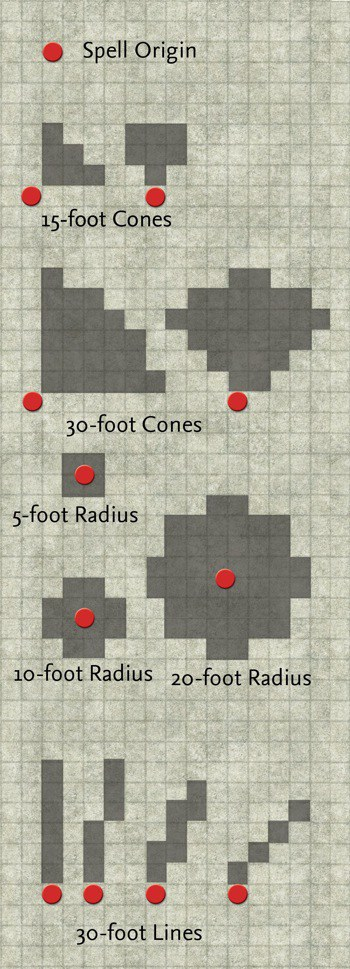
\includegraphics[width=\linewidth]{images/SpellAreas.jpg}
\end{figure}

\textbf{Area}: Some spells affect an area. Sometimes a spell description specifies a specially defined area, but usually an area falls into one of the categories defined below.
				
Regardless of the shape of the area, you select the point where the spell originates, but otherwise you don't control which creatures or objects the spell affects. The point of origin of a spell is always a grid intersection. When determining whether a given creature is within the area of a spell, count out the distance from the point of origin in squares just as you do when moving a character or when determining the range for a ranged attack. The only difference is that instead of counting from the center of one square to the center of the next, you count from intersection to intersection.
				
You can count diagonally across a square, but remember that every second diagonal counts as 2 squares of distance. If the far edge of a square is within the spell's area, anything within that square is within the spell's area. If the spell's area only touches the near edge of a square, however, anything within that square is unaffected by the spell.
				
\textit{Burst, Emanation, or Spread}: Most spells that affect an area function as a burst, an emanation, or a spread. In each case, you select the spell's point of origin and measure its effect from that point.
				
A burst spell affects whatever it catches in its area, including creatures that you can't see. It can't affect creatures with total cover from its point of origin (in other words, its effects don't extend around corners). The default shape for a burst effect is a sphere, but some burst spells are specifically described as cone-shaped. A burst's area defines how far from the point of origin the spell's effect extends.
				
An emanation spell functions like a burst spell, except that the effect continues to radiate from the point of origin for the duration of the spell. Most emanations are cones or spheres.
				
A spread spell extends out like a burst but can turn corners. You select the point of origin, and the spell spreads out a given distance in all directions. Figure the area the spell effect fills by taking into account any turns the spell effect takes.
				
\textit{Cone, Cylinder, Line, or Sphere}: Most spells that affect an area have a particular shape.
				
A cone-shaped spell shoots away from you in a quarter-circle in the direction you designate. It starts from any corner of your square and widens out as it goes. Most cones are either bursts or emanations (see above), and thus won't go around corners.
				
When casting a cylinder-shaped spell, you select the spell's point of origin. This point is the center of a horizontal circle, and the spell shoots down from the circle, filling a cylinder. A cylinder-shaped spell ignores any obstructions within its area.
				
A line-shaped spell shoots away from you in a line in the direction you designate. It starts from any corner of your square and extends to the limit of its range or until it strikes a barrier that blocks line of effect. A line-shaped spell affects all creatures in squares through which the line passes.
				
A sphere-shaped spell expands from its point of origin to fill a spherical area. Spheres may be bursts, emanations, or spreads.
				
\textit{Creatures}: A spell with this kind of area affects creatures directly (like a targeted spell), but it affects all creatures in an area of some kind rather than individual creatures you select. The area might be a spherical burst, a cone-shaped burst, or some other shape.
				
Many spells affect \texttt{{}"{}}living creatures,\texttt{{}"{}} which means all creatures other than constructs and undead. Creatures in the spell's area that are not of the appropriate type do not count against the creatures affected.
				
\textit{Objects}: A spell with this kind of area affects objects within an area you select (as Creatures, but affecting objects instead).
				
\textit{Other}: A spell can have a unique area, as defined in its description.
				
\textit{(S) Shapeable}: If an area or effect entry ends with \texttt{{}"{}}(S),\texttt{{}"{}} you can shape the spell. A shaped effect or area can have no dimension smaller than 10 feet. Many effects or areas are given as cubes to make it easy to model irregular shapes. Three-dimensional volumes are most often needed to define aerial or underwater effects and areas.
				
\textbf{Line of Effect}: A line of effect is a straight, unblocked path that indicates what a spell can affect. A line of effect is canceled by a solid barrier. It's like line of sight for ranged weapons, except that it's not blocked by fog, darkness, and other factors that limit normal sight.
				
You must have a clear line of effect to any target that you cast a spell on or to any space in which you wish to create an effect. You must have a clear line of effect to the point of origin of any spell you cast\textit{.}
				
A burst, cone, cylinder, or emanation spell affects only an area, creature, or object to which it has line of effect from its origin (a spherical burst's center point, a cone-shaped burst's starting point, a cylinder's circle, or an emanation's point of origin).
				
An otherwise solid barrier with a hole of at least 1 square foot through it does not block a spell's line of effect. Such an opening means that the 5-foot length of wall containing the hole is no longer considered a barrier for purposes of a spell's line of effect.
				
\subsection{Duration}

				
A spell's duration entry tells you how long the magical energy of the spell lasts.
				
\textbf{Timed Durations}: Many durations are measured in rounds, minutes, hours, or other increments. When the time is up, the magic goes away and the spell ends. If a spell's duration is variable, the duration is rolled secretly so the caster doesn't know how long the spell will last. 
				
\textbf{Instantaneous}: The spell energy comes and goes the instant the spell is cast, though the consequences might be long-lasting.
				
\textbf{Permanent}: The energy remains as long as the effect does. This means the spell is vulnerable to \textit{dispel magic}. 
				
\textbf{Concentration}: The spell lasts as long as you concentrate on it. Concentrating to maintain a spell is a standard action that does not provoke attacks of opportunity. Anything that could break your concentration when casting a spell can also break your concentration while you're maintaining one, causing the spell to end. See concentration.
				
You can't cast a spell while concentrating on another one. Some spells last for a short time after you cease concentrating.
				
\textbf{Subjects, Effects, and Areas}: If the spell affects creatures directly, the result travels with the subjects for the spell's duration. If the spell creates an effect, the effect lasts for the duration. The effect might move or remain still. Such an effect can be destroyed prior to when its duration ends. If the spell affects an area, then the spell stays with that area for its duration. 
				
Creatures become subject to the spell when they enter the area and are no longer subject to it when they leave.
				
\textbf{Touch Spells and Holding the Charge}: In most cases, if you don't discharge a touch spell on the round you cast it, you can hold the charge (postpone the discharge of the spell) indefinitely. You can make touch attacks round after round until the spell is discharged. If you cast another spell, the touch spell dissipates.
				
Some touch spells allow you to touch multiple targets as part of the spell. You can't hold the charge of such a spell; you must touch all targets of the spell in the same round that you finish casting the spell.
				
\textbf{Discharge}: Occasionally a spells lasts for a set duration or until triggered or discharged.
				
\textbf{(D) Dismissible}: If the duration line ends with \texttt{{}"{}}(D),\texttt{{}"{}} you can dismiss the spell at will. You must be within range of the spell's effect and must speak words of dismissal, which are usually a modified form of the spell's verbal component. If the spell has no verbal component, you can dismiss the effect with a gesture. Dismissing a spell is a standard action that does not provoke attacks of opportunity.
				
A spell that depends on concentration is dismissible by its very nature, and dismissing it does not take an action, since all you have to do to end the spell is to stop concentrating on your turn.
				
\subsection{Saving Throw}

				
Usually a harmful spell allows a target to make a saving throw to avoid some or all of the effect. The saving throw entry in a spell description defines which type of saving throw the spell allows and describes how saving throws against the spell work.
				
\textbf{Negates}: The spell has no effect on a subject that makes a successful saving throw.
				
\textbf{Partial}: The spell has an effect on its subject. A successful saving throw means that some lesser effect occurs.
				
\textbf{Half}: The spell deals damage, and a successful saving throw halves the damage taken (round down).
				
\textbf{None}: No saving throw is allowed.
				
\textbf{Disbelief}: A successful save lets the subject ignore the spell's effect. 
				
\textbf{(object)}: The spell can be cast on objects, which receive saving throws only if they are magical or if they are attended (held, worn, grasped, or the like) by a creature resisting the spell, in which case the object uses the creature's saving throw bonus unless its own bonus is greater. This notation does not mean that a spell can be cast only on objects. Some spells of this sort can be cast on creatures or objects. A magic item's saving throw bonuses are each equal to 2 + 1/2 the item's caster level. 
				
\textbf{(harmless)}: The spell is usually beneficial, not harmful, but a targeted creature can attempt a saving throw if it desires.
				
\textbf{Saving Throw Difficulty Class}: A saving throw against your spell has a DC of 10 + the level of the spell + your bonus for the relevant ability (Intelligence for a wizard, Charisma for a bard, paladin, or sorcerer, or Wisdom for a cleric, druid, or ranger). A spell's level can vary depending on your class. Always use the spell level applicable to your class.
				
\textbf{Succeeding on a Saving Throw}: A creature that successfully saves against a spell that has no obvious physical effects feels a hostile force or a tingle, but cannot deduce the exact nature of the attack. Likewise, if a creature's saving throw succeeds against a targeted spell, you sense that the spell has failed. You do not sense when creatures succeed on saves against effect and area spells.
				
\textbf{Automatic Failures and Successes}: A natural 1 (the d20 comes up 1) on a saving throw is always a failure, and the spell may cause damage to exposed items (see Items Surviving after a Saving Throw, below). A natural 20 (the d20 comes up 20) is always a success.
				
\textbf{Voluntarily Giving up a Saving Throw}: A creature can voluntarily forego a saving throw and willingly accept a spell's result. Even a character with a special resistance to magic can suppress this quality.

\begin{table}[]
\sffamily
\caption{Table: Items Affected by Magical Attacks}
\begin{tabular}{ll}
\textbf{Order*} & \textbf{Item}\\
1st & Shield \\
 2nd & Armor \\
 3rd & Magic helmet, hat, or headband \\
 4th & Item in hand  (including weapon, wand, or the like) \\
 5th & Magic cloak \\
 6th & Stowed or sheathed weapon \\
 7th & Magic bracers \\
 8th & Magic clothing \\
 9th & Magic jewelry (including rings) \\
 10th & Anything else\\
\end{tabular}
* In order of most likely to least likely to be affected.\\
\end{table}

				
\textbf{Items Surviving after a Saving Throw}: Unless the descriptive text for the spell specifies otherwise, all items carried or worn by a creature are assumed to survive a magical attack. If a creature rolls a natural 1 on its saving throw against the effect, however, an exposed item is harmed (if the attack can harm objects). Refer to Table: Items Affected by Magical Attacks. Determine which four objects carried or worn by the creature are most likely to be affected and roll randomly among them. The randomly determined item must make a saving throw against the attack form and take whatever damage the attack dealt.
				
If the selected item is not carried or worn and is not magical, it does not get a saving throw. It simply is dealt the appropriate damage.
				
\subsection{Spell Resistance}

				
Spell resistance is a special defensive ability. If your spell is being resisted by a creature with spell resistance, you must make a caster level check (1d20 + caster level) at least equal to the creature's spell resistance for the spell to affect that creature. The defender's spell resistance is like an Armor Class against magical attacks. Include any adjustments to your caster level to this caster level check.
				
The Spell Resistance entry and the descriptive text of a spell description tell you whether spell resistance protects creatures from the spell. In many cases, spell resistance applies only when a resistant creature is targeted by the spell, not when a resistant creature encounters a spell that is already in place.
				
The terms \texttt{{}"{}}object\texttt{{}"{}} and \texttt{{}"{}}harmless\texttt{{}"{}} mean the same thing for spell resistance as they do for saving throws. A creature with spell resistance must voluntarily lower the resistance (a standard action) in order to be affected by such spells without forcing the caster to make a caster level check.
				
\subsection{Descriptive Text}

				
This portion of a spell description details what the spell does and how it works. If one of the previous entries in the description includes \texttt{{}"{}}see text,\texttt{{}"{}} this is where the explanation is found. 
				
\section{Arcane Spells}

				
Wizards, sorcerers, and bards cast arcane spells. Compared to divine spells, arcane spells are more likely to produce dramatic results.
				
\textbf{Spell Slots}: The various character class tables show how many spells of each level a character can cast per day. These openings for daily spells are called spell slots. A spellcaster always has the option to fill a higher-level spell slot with a lower-level spell. A spellcaster who lacks a high enough ability score to cast spells that would otherwise be his due still gets the slots but must fill them with spells of lower levels.
				
\subsection{Preparing Wizard Spells}

				
A wizard's level limits the number of spells he can prepare and cast. His high Intelligence score might allow him to prepare a few extra spells. He can prepare the same spell more than once, but each preparation counts as one spell toward his daily limit. To prepare a spell, the wizard must have an Intelligence score of at least 10 + the spell's level.
				
\textbf{Rest}: To prepare his daily spells, a wizard must first sleep for 8 hours. The wizard does not have to slumber for every minute of the time, but he must refrain from movement, combat, spellcasting, skill use, conversation, or any other fairly demanding physical or mental task during the rest period. If his rest is interrupted, each interruption adds 1 hour to the total amount of time he has to rest in order to clear his mind, and he must have at least 1 hour of uninterrupted rest immediately prior to preparing his spells. If the character does not need to sleep for some reason, he still must have 8 hours of restful calm before preparing any spells. 
				
\textbf{Recent Casting Limit/Rest Interruptions}: If a wizard has cast spells recently, the drain on his resources reduces his capacity to prepare new spells. When he prepares spells for the coming day, all the spells he has cast within the last 8 hours count against his daily limit.
				
\textbf{Preparation Environment}: To prepare any spell, a wizard must have enough peace, quiet, and comfort to allow for proper concentration. The wizard's surroundings need not be luxurious, but they must be free from distractions. Exposure to inclement weather prevents the necessary concentration, as does any injury or failed saving throw the character might experience while studying. Wizards also must have access to their spellbooks to study from and sufficient light to read them. There is one major exception: a wizard can prepare a \textit{read magic }spell even without a spellbook. 
				
\textbf{Spell Preparation Time}: After resting, a wizard must study his spellbook to prepare any spells that day. If he wants to prepare all his spells, the process takes 1 hour. Preparing some smaller portion of his daily capacity takes a proportionally smaller amount of time, but always at least 15 minutes, the minimum time required to achieve the proper mental state.
				
\textbf{Spell Selection and Preparation}: Until he prepares spells from his spellbook, the only spells a wizard has available to cast are the ones that he already had prepared from the previous day and has not yet used. During the study period, he chooses which spells to prepare. If a wizard already has spells prepared (from the previous day) that he has not cast, she can abandon some or all of them to make room for new spells.
				
When preparing spells for the day, a wizard can leave some of these spell slots open. Later during that day, he can repeat the preparation process as often as he likes, time and circumstances permitting. During these extra sessions of preparation, the wizard can fill these unused spell slots. He cannot, however, abandon a previously prepared spell to replace it with another one or fill a slot that is empty because he has cast a spell in the meantime. That sort of preparation requires a mind fresh from rest. Like the first session of the day, this preparation takes at least 15 minutes, and it takes longer if the wizard prepares more than one-quarter of his spells.
				
\textbf{Prepared Spell Retention}: Once a wizard prepares a spell, it remains in his mind as a nearly cast spell until he uses the prescribed components to complete and trigger it or until he abandons it. Certain other events, such as the effects of magic items or special attacks from monsters, can wipe a prepared spell from a character's mind.
				
\textbf{Death and Prepared Spell Retention}: If a spellcaster dies, all prepared spells stored in his mind are wiped away. Potent magic (such as \textit{raise dead, resurrection, }or \textit{true resurrection}) can recover the lost energy when it recovers the character.
				
\subsection{Arcane Magical Writings}

				
To record an arcane spell in written form, a character uses complex notation that describes the magical forces involved in the spell. The writer uses the same system no matter what her native language or culture. However, each character uses the system in his own way. Another person's magical writing remains incomprehensible to even the most powerful wizard until he takes time to study and decipher it.
				
To decipher an arcane magical writing (such as a single spell in another's spellbook or on a scroll), a character must make a Spellcraft check (DC 20 + the spell's level). If the skill check fails, the character cannot attempt to read that particular spell again until the next day. A \textit{read magic }spell automatically deciphers magical writing without a skill check. If the person who created the magical writing is on hand to help the reader, success is also automatic.
				
Once a character deciphers a particular piece of magical writing, he does not need to decipher it again. Deciphering magical writing allows the reader to identify the spell and gives some idea of its effects (as explained in the spell description). If the magical writing is a scroll and the reader can cast arcane spells, he can attempt to use the scroll.
				
\subsection{Wizard Spells and Borrowed Spellbooks}

				
A wizard can use a borrowed spellbook to prepare a spell he already knows and has recorded in his own spellbook, but preparation success is not assured. First, the wizard must decipher the writing in the book (see Arcane Magical Writings, above). Once a spell from another spellcaster's book is deciphered, the reader must make a Spellcraft check (DC 15 + spell's level) to prepare the spell. If the check succeeds, the wizard can prepare the spell. He must repeat the check to prepare the spell again, no matter how many times he has prepared it before. If the check fails, he cannot try to prepare the spell from the same source again until the next day. However, as explained above, he does not need to repeat a check to decipher the writing.
				
\subsection{Adding Spells to a Wizard's Spellbook}

				
Wizards can add new spells to their spellbooks through several methods. A wizard can only learn new spells that belong to the wizard spell lists.
				
\textbf{Spells Gained at a New Level}: Wizards perform a certain amount of spell research between adventures. Each time a character attains a new wizard level, he gains two spells of his choice to add to his spellbook. The two free spells must be of spell levels he can cast.
				
\textbf{Spells Copied from Another's Spellbook or a Scroll}: A wizard can also add a spell to his book whenever he encounters one on a magic scroll or in another wizard's spellbook. No matter what the spell's source, the wizard must first decipher the magical writing (see Arcane Magical Writings). Next, he must spend 1 hour studying the spell. At the end of the hour, he must make a Spellcraft check (DC 15 + spell's level). A wizard who has specialized in a school of spells gains a +2 bonus on the Spellcraft check if the new spell is from his specialty school. If the check succeeds, the wizard understands the spell and can copy it into his spellbook (see Writing a New Spell into a Spellbook). The process leaves a spellbook that was copied from unharmed, but a spell successfully copied from a magic scroll disappears from the parchment.
				
If the check fails, the wizard cannot understand or copy the spell. He cannot attempt to learn or copy that spell again until one week has passed. If the spell was from a scroll, a failed Spellcraft check does not cause the spell to vanish.
				
In most cases, wizards charge a fee for the privilege of copying spells from their spellbooks. This fee is usually equal to half the cost to write the spell into a spellbook (see Writing a New Spell into a Spellbook). Rare and unique spells might cost significantly more.
				
\textbf{Independent Research}: A wizard can also research a spell independently, duplicating an existing spell or creating an entirely new one. The cost to research a new spell, and the time required, are left up to GM discretion, but it should probably take at least 1 week and cost at least 1,000 gp per level of the spell to be researched. This should also require a number of Spellcraft and Knowledge (arcana) checks.
				
\subsection{Writing a New Spell into a Spellbook}

				
Once a wizard understands a new spell, he can record it into his spellbook.
				
\textbf{Time}: The process takes 1 hour per spell level. Cantrips (0 levels spells) take 30 minutes to record.
				
\textbf{Space in the Spellbook}: A spell takes up one page of the spellbook per spell level. Even a 0-level spell (cantrip) takes one page. A spellbook has 100 pages.
				
\textbf{Materials and Costs}: The cost for writing a new spell into a spellbook depends on the level of the spell, as noted on the following table. Note that a wizard does not have to pay these costs in time or gold for spells he gains for free at each new level.

\begin{table}
\sffamily
 \begin{tabular}{ll}
\textbf{Spell Level} & \textbf{Writing Cost}\\
0 & 5 gp\\
1 & 10 gp\\
2 & 40 gp\\
3 & 90 gp\\
4 & 160 gp\\
5 & 250 gp\\
6 & 360 gp\\
7 & 490 gp\\
8 & 640 gp\\
9 & 810 gp\\
 \end{tabular}

\end{table}

% </tbody id="writing-a-new-spell-into-a-spellbook-69">

				
\subsection{Replacing and Copying Spellbooks}

				
A wizard can use the procedure for learning a spell to reconstruct a lost spellbook. If he already has a particular spell prepared, he can write it directly into a new book at the same cost required to write a spell into a spellbook. The process wipes the prepared spell from his mind, just as casting it would. If he does not have the spell prepared, he can prepare it from a borrowed spellbook and then write it into a new book.
				
Duplicating an existing spellbook uses the same procedure as replacing it, but the task is much easier. The time requirement and cost per page are halved.
				
\subsection{Selling a Spellbook}

				
Captured spellbooks can be sold for an amount equal to half the cost of purchasing and inscribing the spells within.
				
\subsection{Sorcerers and Bards}

				
Sorcerers and bards cast arcane spells, but they do not use spellbooks or prepare spells. Their class level limits the number of spells she can cast (see these class descriptions). Her high Charisma score might allow her to cast a few extra spells. A member of either class must have a Charisma score of at least 10 + the spell's level to cast the spell.
				
\textbf{Daily Readying of Spells}: Each day, sorcerers and bards must focus their minds on the task of casting their spells. A sorcerer or bard needs 8 hours of rest (just like a wizard), after which she spends 15 minutes concentrating. (A bard must sing, recite, or play an instrument of some kind while concentrating.) During this period, the sorcerer or bard readies her mind to cast her daily allotment of spells. Without such a period to refresh herself, the character does not regain the spell slots she used up the day before.
				
\textbf{Recent Casting Limit}: Any spells cast within the last 8 hours count against the sorcerer's or bard's daily limit.
				
\textbf{Adding Spells to a Sorcerer's or Bard's Repertoire}: A sorcerer or bard gains spells each time she attains a new level in her class and never gains spells any other way. When your sorcerer or bard gains a new level, consult Table: Bard Spells Known or Table: Sorcerer Spells Known to learn how many spells from the appropriate spell list she now knows. With permission from the GM, sorcerers and bards can also select the spells they gain from new and unusual spells that they come across while adventuring.
				
\section{Divine Spells}

				
Clerics, druids, experienced paladins, and experienced rangers can cast divine spells. Unlike arcane spells, divine spells draw power from a divine source. Clerics gain spell power from deities or from divine forces. The divine force of nature powers druid and ranger spells, and the divine forces of law and good power paladin spells. Divine spells tend to focus on healing and protection and are less flashy, destructive, and disruptive than arcane spells.
				
\subsection{Preparing Divine Spells}

				
Divine spellcasters prepare their spells in largely the same manner as wizards do, but with a few differences. The relevant ability for most divine spells is Wisdom (Charisma for paladins). To prepare a divine spell, a character must have a Wisdom score (or Charisma score for paladins) of 10 + the spell's level. Likewise, bonus spells are based on Wisdom.
				
\textbf{Time of Day}: A divine spellcaster chooses and prepares spells ahead of time, but unlike a wizard, does not require a period of rest to prepare spells. Instead, the character chooses a particular time of day to pray and receive spells. The time is usually associated with some daily event. If some event prevents a character from praying at the proper time, she must do so as soon as possible. If the character does not stop to pray for spells at the first opportunity, she must wait until the next day to prepare spells.
				
\textbf{Spell Selection and Preparation}: A divine spellcaster selects and prepares spells ahead of time through prayer and meditation at a particular time of day. The time required to prepare spells is the same as it is for a wizard (1 hour), as is the requirement for a relatively peaceful environment. When preparing spells for the day, a cleric can leave some of her spell slots open. Later during that day, she can repeat the preparation process as often as she likes. During these extra sessions of preparation, she can fill these unused spell slots. She cannot, however, abandon a previously prepared spell to replace it with another one or fill a slot that is empty because she has cast a spell in the meantime. Like the first session of the day, this preparation takes at least 15 minutes, and it takes longer if she prepares more than one-quarter of his spells.
				
Divine spellcasters do not require spellbooks. However, a divine spellcaster's spell selection is limited to the spells on the list for her class. Clerics, druids, paladins, and rangers have separate spell lists. A cleric also has access to two domains determined during character creation. Each domain gives her access to a number of special abilities and bonus spells.
				
\textbf{Spell Slots}: The character class tables show how many spells of each level each can cast per day. These openings for daily spells are called spell slots. A spellcaster always has the option to fill a higher-level spell slot with a lower-level spell. A spellcaster who lacks a high enough ability score to cast spells that would otherwise be her due still gets the slots but must fill them with spells of lower levels. 
				
\textbf{Recent Casting Limit}: As with arcane spells, at the time of preparation any spells cast within the previous 8 hours count against the number of spells that can be prepared.
				
\textbf{Spontaneous Casting of Cure} \textbf{and Inflict} \textbf{Spells}: A good cleric (or a cleric of a good deity) can spontaneously cast a cure spell in place of a prepared spell of the same level or higher, but not in place of a bonus domain spell. An evil cleric (or a cleric of an evil deity) can spontaneously cast an inflict spell in place of a prepared spell (that is not a domain spell) of the same level or higher. Each neutral cleric of a neutral deity spontaneously casts either cure spells like a good cleric or inflict spells like an evil one, depending on which option the player chooses when creating the character. The divine energy of the spell that the cure or inflict spell substitutes for is converted into the cure or inflict spell as if that spell had been prepared all along.
				
\textbf{Spontaneous Casting of  \textit{Summon Nature's Ally } Spells}: A druid can spontaneously cast \textit{summon nature's ally }in place of a prepared spell of the same level or higher. The divine energy of the spell that the summon spell substitutes for is converted as if that spell had been prepared all along.
				
\subsection{Divine Magical Writings}

				
Divine spells can be written and deciphered like arcane spells (see Arcane Magical Writings). A Spellcraft check can decipher divine magical writing and identify it. Only characters who have the spell (in its divine form) on their class spell list can cast a divine spell from a scroll.
				
\subsection{New Divine Spells}

				
Divine spellcasters gain new spells as follows.
				
\textbf{Spells Gained at a New Level}: Characters who can cast divine spells undertake a certain amount of study between adventures. Each time such a character receives a new level of divine spells, she learns all of the spells from that level automatically.
				
\textbf{Independent Research}: A divine spellcaster can also research a spell independently, much as an arcane spellcaster can. Only the creator of such a spell can prepare and cast it, unless she decides to share it with others.
				
\section{Special Abilities}

				
A number of classes and creatures gain the use of special abilities, many of which function like spells.
				
\textbf{Spell-Like Abilities}: Usually, a spell-like ability works just like the spell of that name. A spell-like ability has no verbal, somatic, or material component, nor does it require a focus. The user activates it mentally. Armor never affects a spell-like ability's use, even if the ability resembles an arcane spell with a somatic component.
				
A spell-like ability has a casting time of 1 standard action unless noted otherwise in the ability or spell description. In all other ways, a spell-like ability functions just like a spell.
				
Spell-like abilities are subject to spell resistance and \textit{dispel magic}. They do not function in areas where magic is suppressed or negated. Spell-like abilities cannot be used to counterspell, nor can they be counterspelled.
				
If a character class grants a spell-like ability that is not based on an actual spell, the ability's effective spell level is equal to the highest-level class spell the character can cast, and is cast at the class level the ability is granted.
				
\textbf{Supernatural Abilities}: These can't be disrupted in combat and generally don't provoke attacks of opportunity. They aren't subject to spell resistance, counterspells, or \textit{dispel magic}, and don't function in antimagic areas.
				
\textbf{Extraordinary Abilities}: These abilities cannot be disrupted in combat, as spells can, and they generally do not provoke attacks of opportunity. Effects or areas that negate or disrupt magic have no effect on extraordinary abilities. They are not subject to dispelling, and they function normally in an \textit{antimagic field. }Indeed, extraordinary abilities do not qualify as magical, though they may break the laws of physics.
				
\textbf{Natural Abilities}: This category includes abilities a creature has because of its physical nature. Natural abilities are those not otherwise designated as extraordinary, supernatural, or spell-like.
